% Chapter 2

\chapter{Resultados} % Main chapter title

\label{Chap:Res} % For referencing the chapter elsewhere, use \ref{Chapter2} 

\section{Introducción}

En este capítulo se presentarán los procedimientos requeridos para llevar a cabo el experimento descrito en el capítulo anterior, y se expondrán los resultados obtenidos de realizar las mediciones. Posteriormente, se mostrarán gráficas de los datos obtenidos con una explicación de sus componentes y su respectiva interpretación. \\

\section{Dibujo del plano}

Para el trazo de la figura cuadrado, que será de 15 metros por lado, se utilizaron dos varas unidas por una fracción de rafia como las de la figura~\ref{fig:HerTraz}, utilizados para el trazado de las circunferencias necesarias.\\

\begin{figure}[H]
\centering
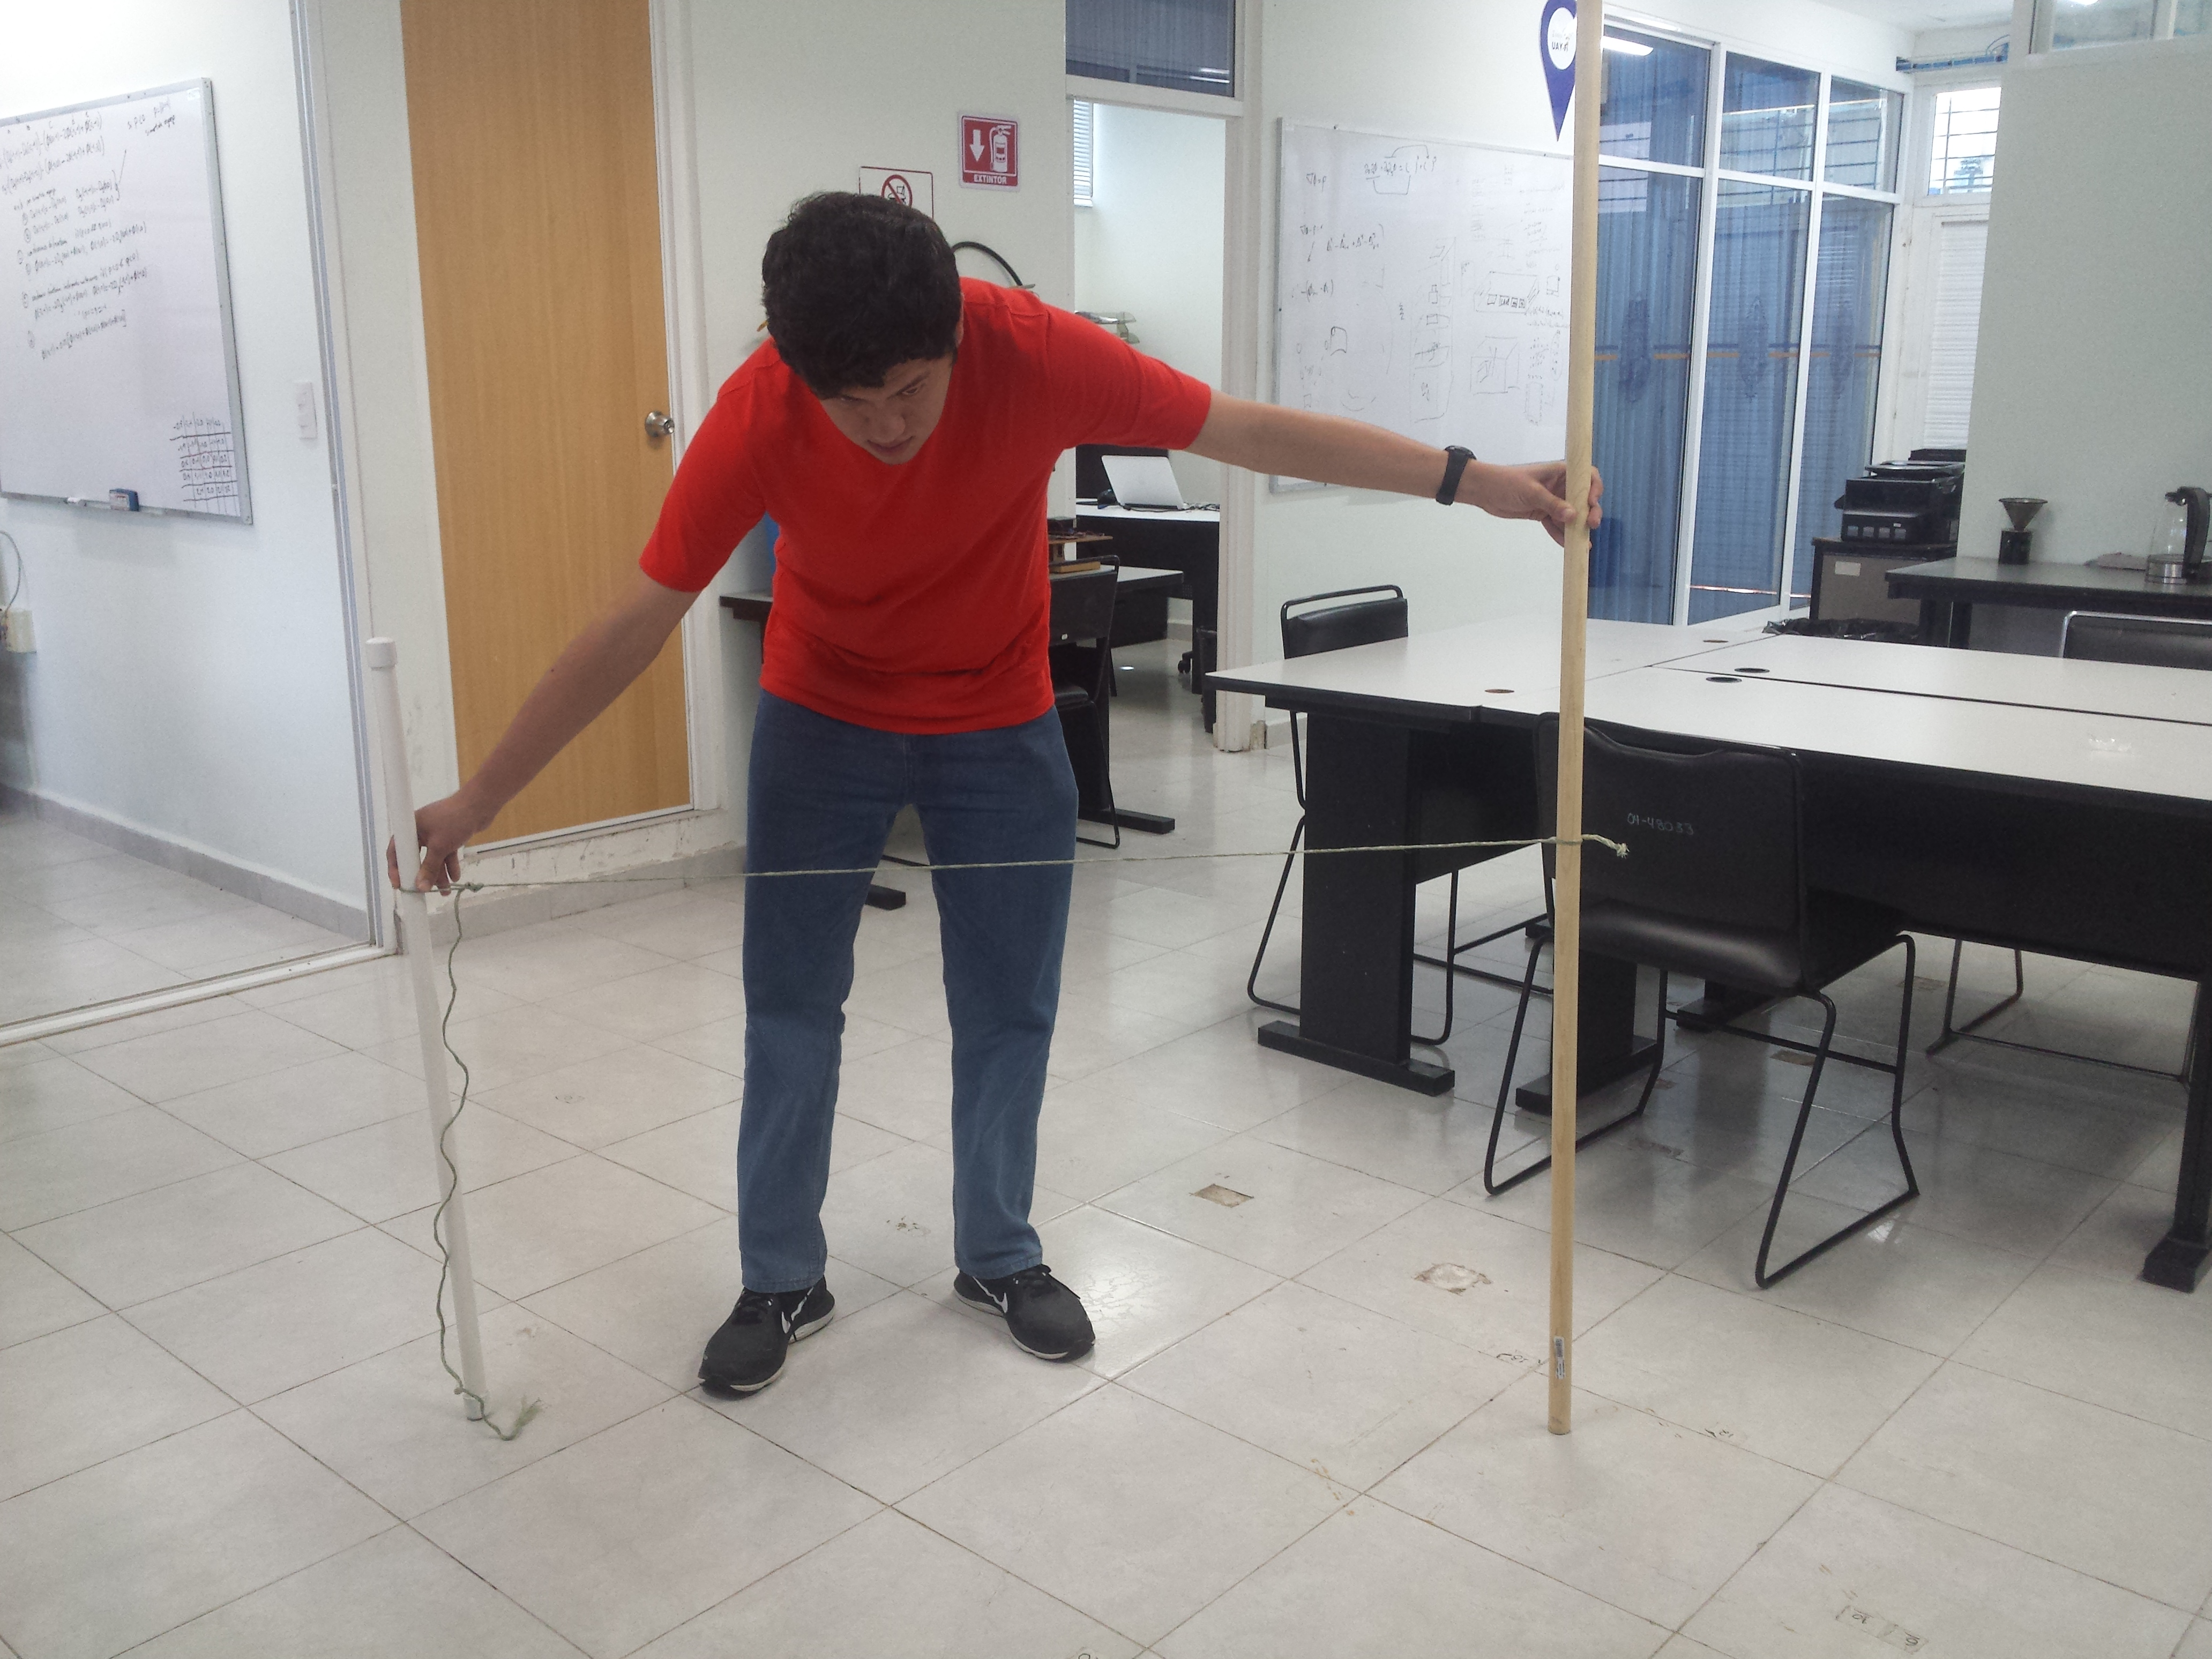
\includegraphics[width=0.95\textwidth]{Figures/Herr}
\caption[Herramientas de trazado.]{Herramientas de trazado.}
\label{fig:HerTraz}
\end{figure}

Para garantizar que se trace una línea recta en cada uno de los lados de la figura, se utilizó una cuerda de nailon de 17 metros de longitud, que una vez tensa, permitió realizar las marcas equidistantes cada 3 metros con un flexómetro, signos en el suelo como los de la figura~\ref{fig:MarEq}.

\begin{figure}[H]
\centering
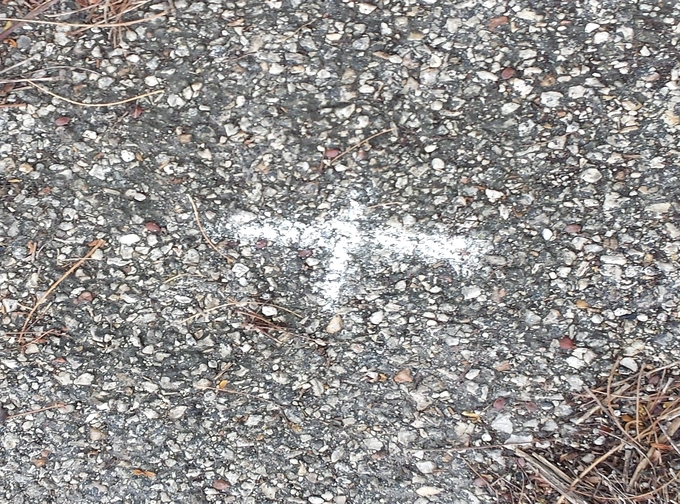
\includegraphics[width=0.95\textwidth]{Figures/Equid}
\caption[Marcas equidistantes en el suelo.]{Marcas equidistantes en el suelo.}
\label{fig:MarEq}
\end{figure}

\section{Mediciones}

\begin{figure}[H]
\centering
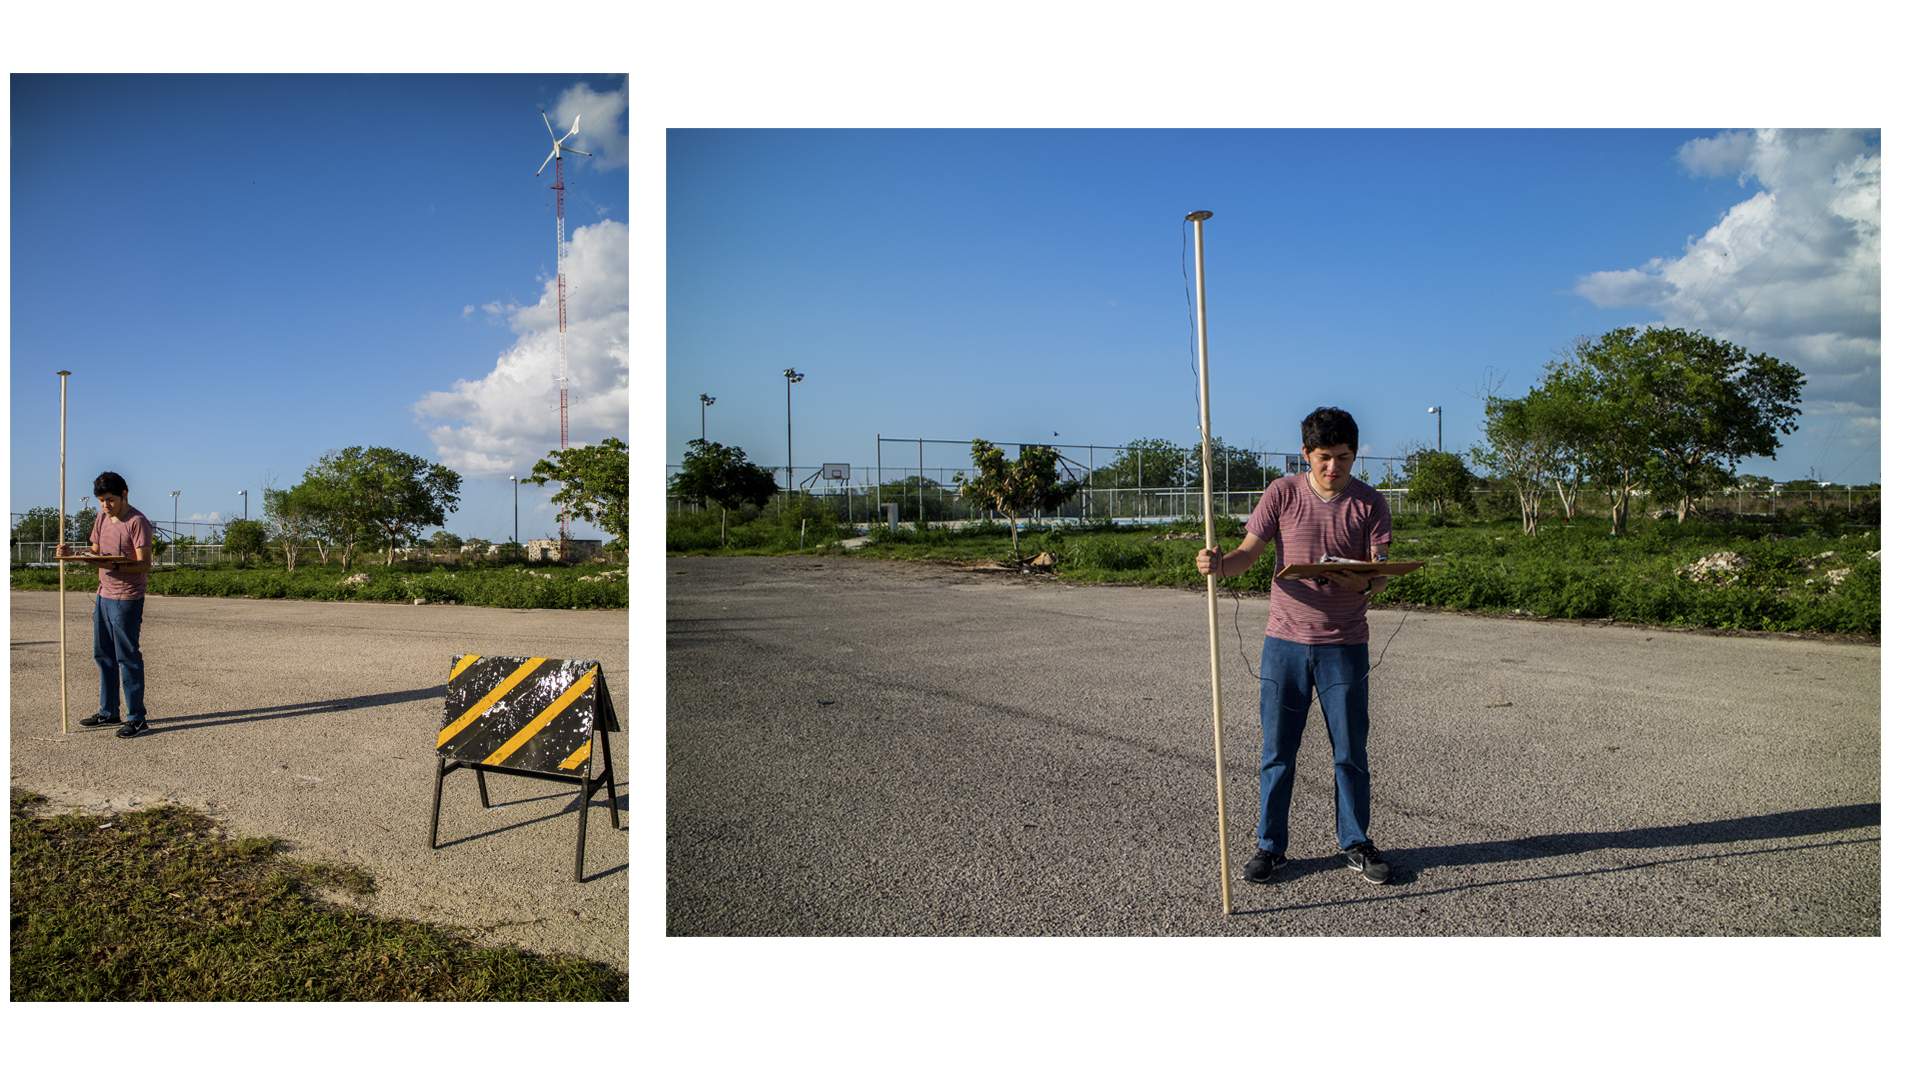
\includegraphics[width=0.95\textwidth]{Figures/22jpg}
\caption[Toma de muestras de coordenadas.]{Toma de muestras de coordenadas.}
\label{fig:Medc}
\end{figure}

Una vez finalizada la separación en 5 segmentos por cada lado de la figura, de 3 metros de separación entre ellos, se obtienen 6 puntos de medición; tras ser configuradas ambas estaciones, se procedió a realizar las mediciones de las coordenadas en los puntos. En la figura~\ref{fig:Medc} se muestran diversos momentos de la toma de muestras correspondientes a las mostradas en este capítulo. Puede observarse un cielo en su mayor parte despejado. Se decidió tomar muestras tanto en el modo Real-Time Kinematics como con el modo de un solo GPS sin retroalimentación de una estación base para comparar resultados. En ambos modos, se recorrió el trazado de la figura dos veces con la antena, en dos sentidos diferentes, llegando a obtener dos mediciones de coordenadas por punto en cada modo de funcionamiento.\\

\begin{figure}[H]
\centering
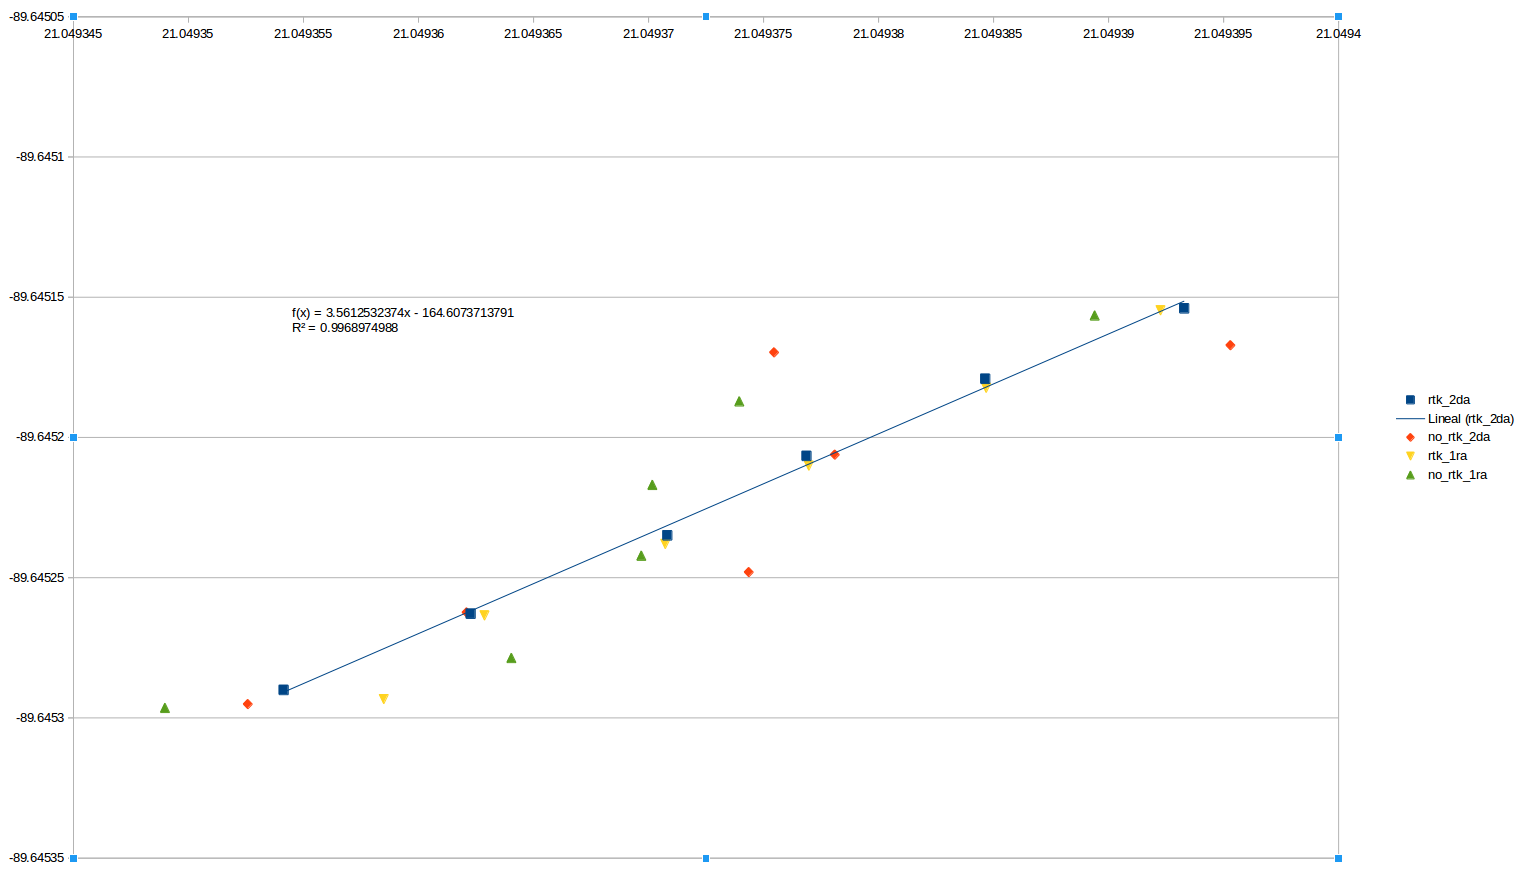
\includegraphics[width=1\textwidth]{Figures/Dispers}
\caption[Diagrama de dispersión de datos registrados en las marcas del lado sur de la figura.]{Diagrama de dispersión de coordenadas registradas en las marcas del lado sur de la figura.}
\label{fig:Disp}
\end{figure}

En la figura~\ref{fig:Disp} se comparan las mediciones realizadas en las marcas del lado sur de la figura, mediante una regresión lineal utilizando los puntos del segundo recorrido en el modo Real-Time Kinematics. Los cuadrados azules marcan el segundo recorrido de muestreo de la figura realizado en el modo Real-Time Kinematics. Los triángulos amarillos marcan las muestras del primer recorrido de muestreo en el mismo modo. El rombo rojo y el triángulo verde marcan el mismo orden pero del modo con un sólo GPS sin retroalimentación de posicionamiento.\\

\newpage

Las muestras realizadas en el modo Real-Time Kinematics muestran, en su segundo recorrido, marcado con cuadros azules, un mayor ajuste a la línea recta de la figura, donde el valor del coeficiente de correlación múltiple $R^{2} \approx 0.997$\footnotemark sugiere un alto ajuste a una línea recta. En el primer recorrido, marcado con triángulos amarillos, se puede observar la misma tendencia pero con un menor ajuste. El resto de puntos, marcados con círculos rojos y triángulos verdes, son en un modo sin Real-Time Kinematics y se puede observar que el ajuste a una línea recta es mucho menor que el modo RTK, llegando a tener variaciones bastante considerables respecto a dicho método.\\

\footnotetext{El valor de $R^{2}$ varía de 0 a 1. Mientras más cerca esté su valor de la unidad, se sugiere una correlación más alta a la recta en este caso. Las muestras escogidas para realizar este cálculo fueron las que se realizaron con Real-Time Kinematics durante la segunda vuelta.}

En el modo Real-Time Kinematics, en cada muestra, existe un valor denominado \textit{ratio} que indica la calidad de la señal de los satélites y de las mediciones del GPS en el \textit{rover} de forma proporcional. En otras palabras, mientras más alto sea el valor de ratio, mucha mejor será la corrección de la señal de GPS. En la figura~\ref{fig:Ratio} se observa cómo en las primeras muestras, el valor del \textit{ratio} oscilaba en valores bajos (se consideran valores bajos aquellos que están debajo de 3). Conforme el tiempo avanzaba, se captaban más satélites y, como consecuencia, el valor del \textit{ratio} ascendió a valores altos. Este comportamiento se ajusta a la gráfica de dispersión en la figura~\ref{fig:Disp}, que muestra que en el primer recorrido, denotado con un triángulo amarillo, el primer punto muestreado (el que está más a la izquierda) estuvo algo más separado de la recta que el resto de muestras en el mismo modo de funcionamiento.

\begin{figure}[H]
\centering
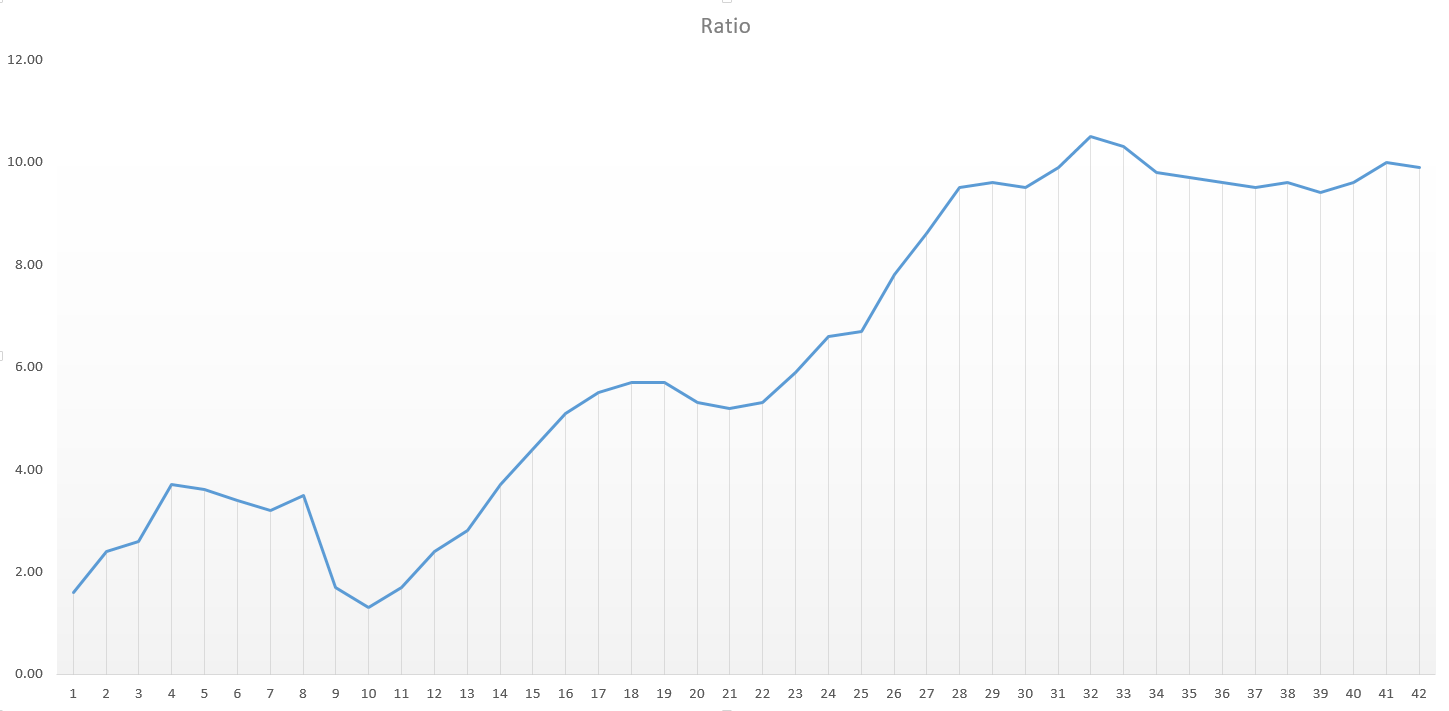
\includegraphics[width=1\textwidth]{Figures/Ratio}
\caption[Gráfica del ratio (confianza de los datos presentados).]{Gráfica del ratio (confianza de los datos presentados).}
\label{fig:Ratio}
\end{figure}

Para obtener el error en metros de las mediciones, se calculó la diferencia existente en distancia entre dos puntos marcados para realizar muestras de coordenadas correspondientes al mismo lado del cuadrado. Todas las coordenadas tomadas para estos cálculos son los correspondientes a la segunda vuelta de cada modalidad. El punto de origen fue el vértice inferior izquierdo y las distancias fueron tomadas en el sentido de las agujas del reloj. Así, el segmento 1 corresponderá a la distancia entre el origen, y el primer punto a 3 metros de él que se ubica en el lado izquierdo de la figura. El segmento 2 corresponderá a la distancia entre el primer y segundo punto en el lado izquierdo del cuadrado, y así sucesivamente. Cada par de puntos deben tener una diferencia existente de tres metros entre sí. Por tanto, se calculó la diferencia en metros a partir de las coordenadas obtenidas, datos mostrados en la figura~\ref{fig:ErrMts}. 

\begin{figure}[H]
\centering
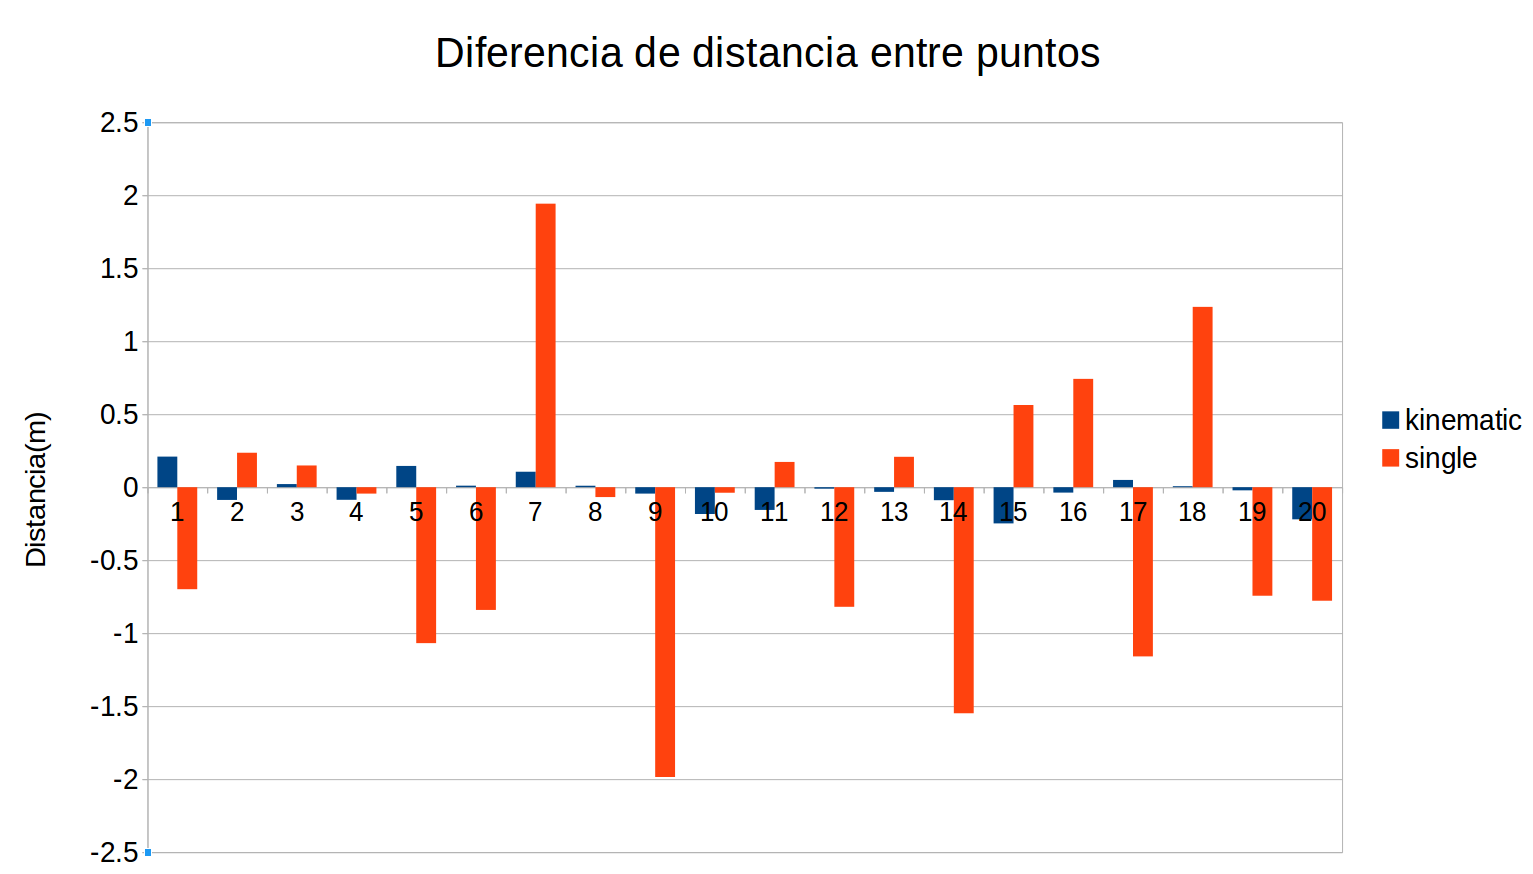
\includegraphics[width=0.95\textwidth]{Figures/ErrMts}
\caption[Diferencia entre la distancia medida entre puntos y la distancia nominal de 3 metros por segmento.]{Diferencia entre la distancia medida entre puntos y la distancia nominal de 3 metros por segmento.}
\label{fig:ErrMts}
\end{figure}

El error promedio obtenido en ambas modalidades se muestra en la figura~\ref{fig:ErrProm}. En modo \textbf{Real-Time Kinematics}, se obtuvo un error promedio de \textbf{$\pm 0.08876$} metros, en contraste al modo sin retroalimentación o \textbf{Single}, donde se obtuvo un error promedio de \textbf{$\pm 0.752035$} metros.

\begin{figure}[H]
\centering
\includegraphics[width=0.95\textwidth]{Figures/ErrProm}
\caption[Diferencia entre la distancia medida entre puntos y la distancia nominal de 3 metros por segmento.]{Diferencia entre la distancia medida entre puntos y la distancia nominal de 3 metros por segmento.}
\label{fig:ErrProm}
\end{figure}

Finalmente, las coordenadas obtenidas durante la rutina se muestran en el mapa en las figuras~\ref{fig:NoRtkRes}~y~\ref{fig:RtkRes}, siendo la primera la solución sin retroalimentación y la segunda la solución con RTK.

\begin{figure}[H]
\centering
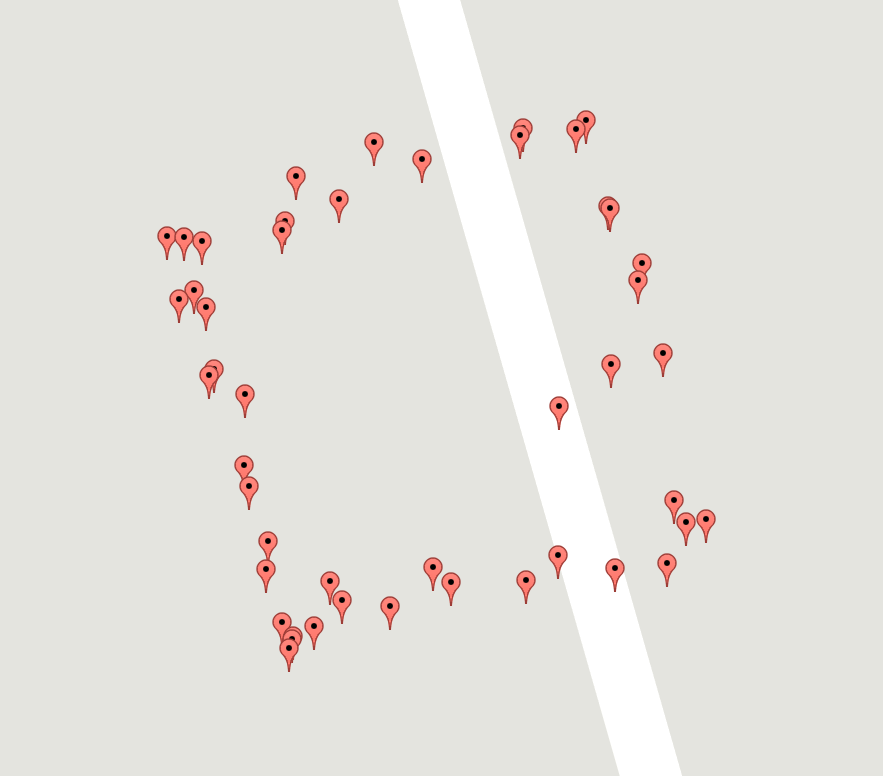
\includegraphics[width=0.8\textwidth]{Figures/NoRtkRes}
\caption[Muestras obtenidas sin Real-Time Kinematics.]{Muestras obtenidas por el sistema sin Real-Time Kinematics.}
\label{fig:NoRtkRes}
\end{figure}

\begin{figure}[H]
\centering
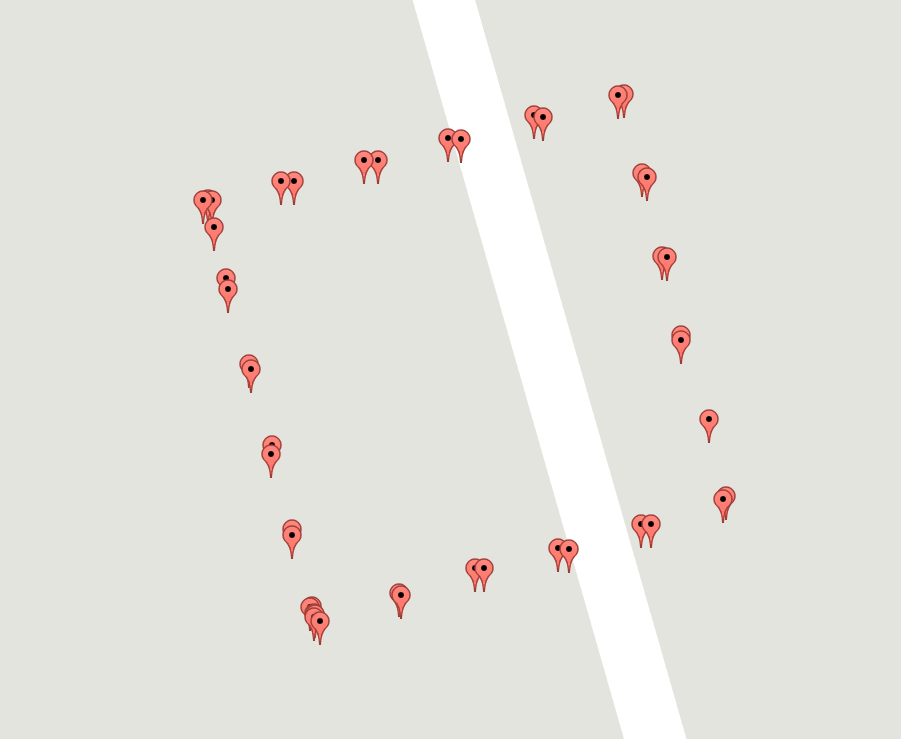
\includegraphics[width=0.8\textwidth]{Figures/RtkRes}
\caption[Muestras obtenidas por el sistema con Real-Time Kinematics.]{Muestras obtenidas por el sistema \textbf{con Real-Time Kinematics}.}
\label{fig:RtkRes}
\end{figure}

Nótese cómo en la solución sin retroalimentación (figura~\ref{fig:NoRtkRes}) se muestran variaciones muy altas en las líneas rectas que conforman el cuadrado, y las muestras se ven afectadas notoriamente en el lado este de la figura. Por otro lado, en la solución con RTK se muestra un mucho mejor ajuste a los puntos marcados y se observa un mejor acoplamiento a la forma del cuadrado.

\section{Conclusión}
Tras el análisis de los resultados, se determinó que la solución con Real-Time Kinematics ayuda a mantener la estabilidad de las mediciones de GPS, siendo 8.47 veces más precisa que la solución Single, pudiendo determinar mejor la posición de los puntos al realizar un recorrido de una rutina previamente estructurada.